\documentclass[a4paper]{report}
\usepackage{float}
\usepackage{verbatim}
\usepackage[utf8]{inputenc}
\usepackage[italian]{babel}
\usepackage{amsmath}
\usepackage{mathtools}
\usepackage{amsbsy,amssymb,amsfonts, amsthm, mhchem, multicol}
\usepackage{graphicx}
\usepackage[left=2cm,right=2cm,top=2cm,bottom=2cm]{geometry}
\usepackage{xcolor}
\usepackage[hypertexnames=false]{hyperref}
\usepackage{nameref}
\usepackage{framed}
\usepackage[framemethod=TikZ]{mdframed}

% figure support
\usepackage{import}
\usepackage{xifthen}
\pdfminorversion=7
\usepackage{pdfpages}
\usepackage{transparent}
\newcommand{\incfig}[1]{%
    \def\svgwidth{\columnwidth}
    \import{./figures/}{#1.pdf_tex}
}
\newcommand{\ffrac}[2]{\ensuremath{\frac{\displaystyle #1}{\displaystyle #2}}}
\newcommand{\angstrom}{\mbox{\normalfont\AA}}
\newcommand{\vect}[1]{\boldsymbol{#1}}
\renewcommand{\[}{\begin{equation}}
\renewcommand{\]}{\end{equation}}
\renewcommand{\theequation}{\thesection.\arabic{equation}}
\counterwithin*{equation}{section}
\newcommand{\rom}[1]{\uppercase\expandafter{\romannumeral #1\relax}}
% title setup
\makeatother
\def\@lez{}%
\newcommand{\lez}[3]{
    \ifthenelse{\isempty{#3}}{%
	\def\@lez{Lezione #1}%
    }{%
	\def\@lez{Lezione #1: #3}%
    }%
    \section{\@lez}
    \marginpar{\small\textsf{\mbox{#2}}}
}
\makeatletter

\definecolor{mygreen}{rgb}{0.0, 0.4, 0.}
\newtheoremstyle{break}%
	{1em}{1em}%
	{}{}%
	{\bfseries}{}% % Note that final punctuation is omitted.
	{\newline}
	{#1 #2: \normalfont(\textcolor{mygreen}{#3})}

\newtheoremstyle{defn}
	{\topsep}   % ABOVESPACE
	{\topsep}   % BELOWSPACE
	{\itshape}  % BODYFONT
	{0pt}       % INDENT (empty value is the same as 0pt)
	{\bfseries} % HEADFONT
	{.}         % HEADPUNCT
	{5pt plus 1pt minus 1pt} % HEADSPACE
	{#1 #2: \normalfont(\textcolor{red}{#3})}          % CUSTOM-HEAD-SPEC

\newtheoremstyle{thm}% name of the style to be used
	{\topsep}% measure of space to leave above the theorem. E.g.: 3pt
	{\topsep}% measure of space to leave below the theorem. E.g.: 3pt
	{\itshape}% name of font to use in the body of the theorem
	{0pt}% measure of space to indent
	{\bfseries}% name of head font
	{.}% punctuation between head and body
	{ }% space after theorem head; " " = normal interword space
	{#1 #2: \normalfont(\textcolor{red}{\underline{#3}})}

\theoremstyle{thm}
\newtheorem{thm}{Teorema}[section] % reset theorem numbering for each chapter

\theoremstyle{defn}
\newtheorem{defn}{Definizione}[section] % definition numbers are dependent on theorem numbers

\theoremstyle{break}
\newtheorem{exmp}{Esempio}[section]
\newtheorem{ex}{Esercizio}[section] % definition numbers are dependent on theorem numbers

\author{Edoardo Gabrielli}
\title{Eserciziario di Dinamica Non Lineare}
\begin{document}
\maketitle 
\tableofcontents
\chapter{Introduzione ai sistemi dinamici}
\begin{ex}[]
    Sia dato l'oscillatore smorzato 
    \[
	\frac{\text{d} ^2x}{\text{d} t^2} + \alpha\frac{\text{d} x}{\text{d} t} + x = 0 \quad  (\alpha >0) 
    .\] 
    Dimostrare che l'unico stato non-Wandering è $\v{V}_s = \begin{pmatrix} 0 \\ 0\end{pmatrix}$.
\end{ex}
\noindent
\begin{ex}[]
    Dato l'oscillatore
    \[
        \frac{\text{d} ^2x}{\text{d} t^2} + x
    .\] 
    Dimostrare che qualunque stato $\v{P}\in \mathbb{R}^n$ è non-Wandering.
\end{ex}
\noindent

\section{Esistenza ed unicità delle soluzioni di un IVP}%
\begin{ex}[Studio di IVP 1]
    Studiare al variare del parametro $x_0$  il seguente IVP:
    \[
        \begin{cases}
            \frac{\text{d} x}{\text{d} t} = x^2\\
	    x(0) = x_0
        \end{cases}
    \] 
\end{ex}
\noindent
\begin{ex}[Studio di IVP 2]
    Studiare al variare del parametro $a$ il seguente IVP:
    \[
        \begin{cases}
            \frac{\text{d} x}{\text{d} t} = \sqrt{x} \\
	    x(0)=a
        \end{cases}
    \] 
\end{ex}
\noindent


\setcounter{section}{3}
\section{Mappe ricorsive}%
\begin{ex}[Sulla mappa di Arnold]
       Dimostrare che la mappa di Arnold è invertibile se $0\le k\le 1$.
\end{ex}
\noindent
\paragraph{Soluzione}%
       \begin{figure}[H]
           \centering
           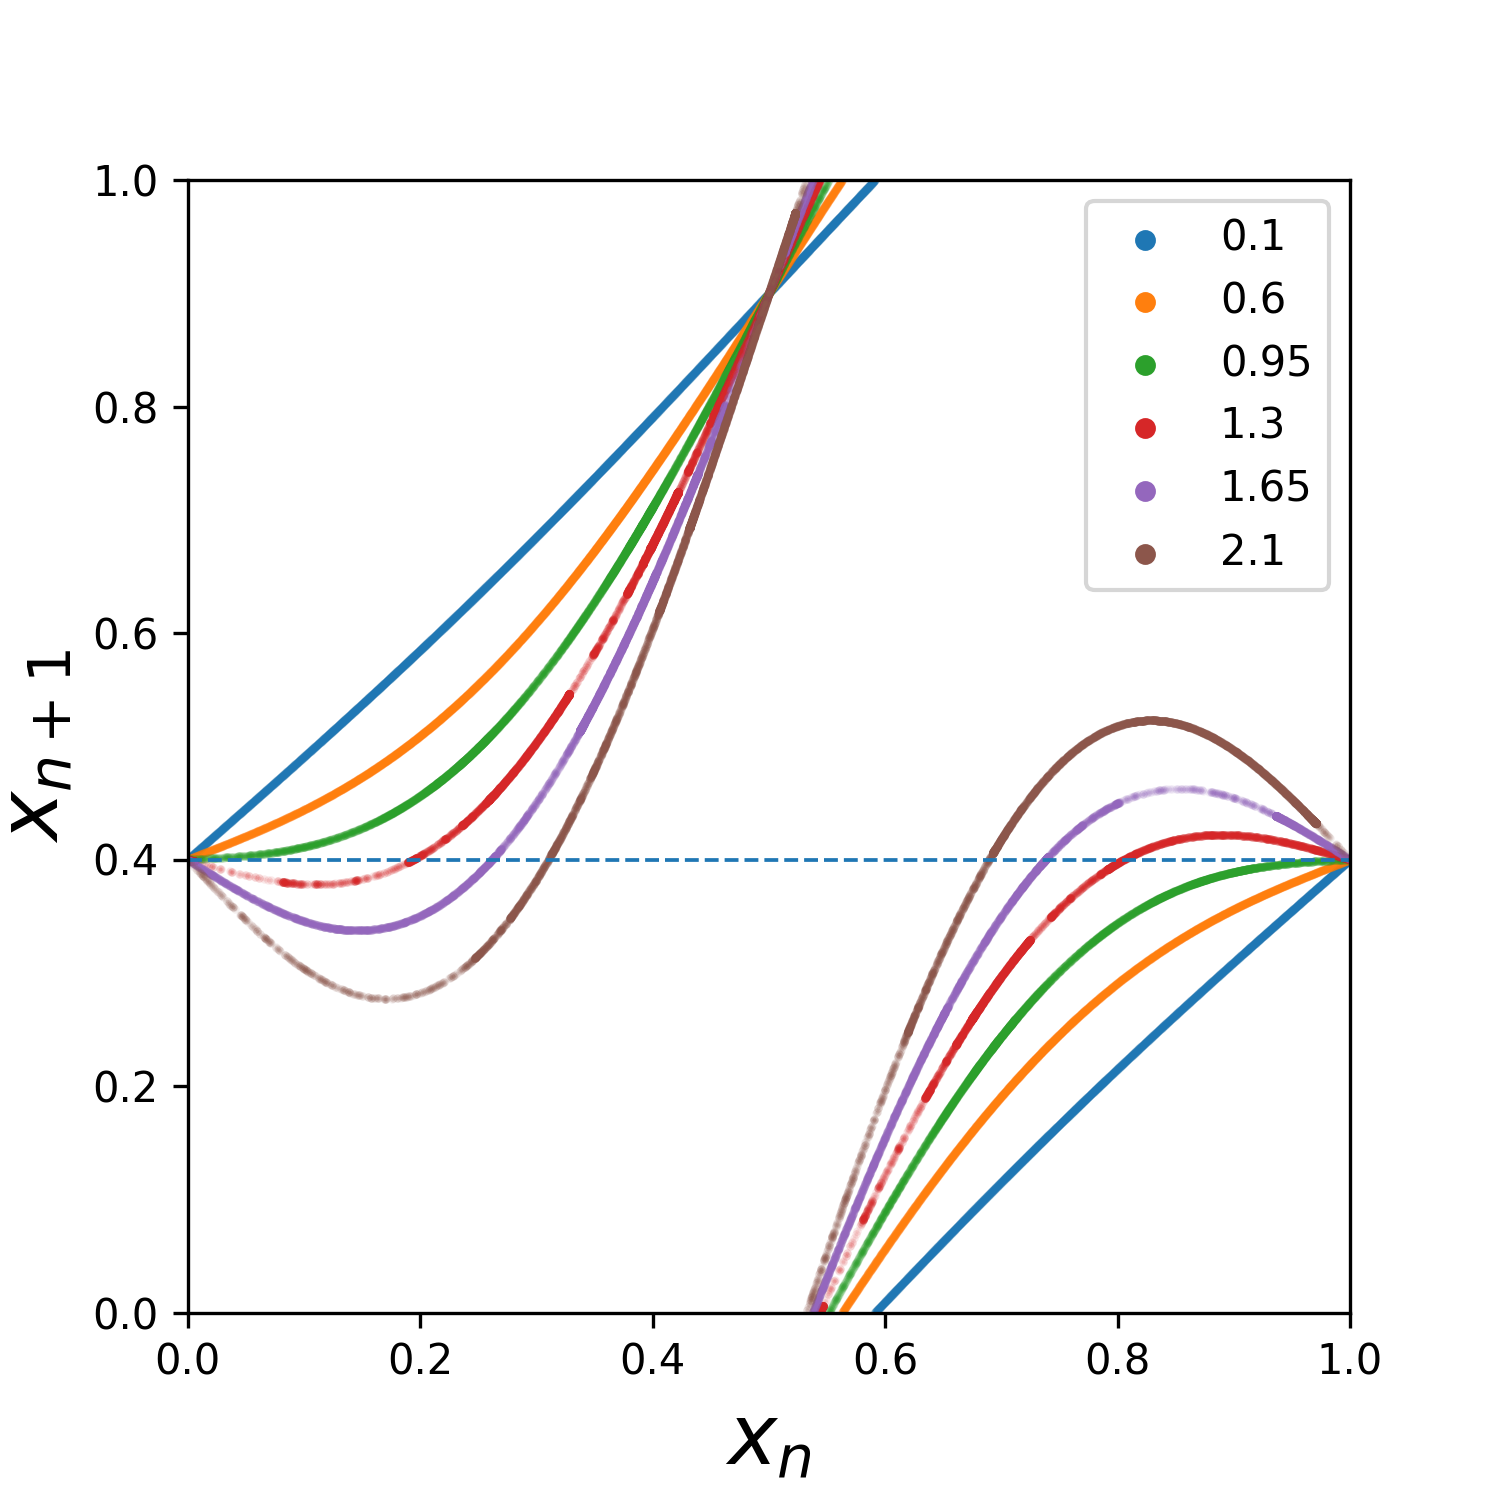
\includegraphics[width=0.3\textwidth]{../figures/chap1/4_3_py.png}
	   \caption{\scriptsize Mappa di Arnold al variare di $k$ con $\omega  = 0.4$ fissato.}
           \label{fig:4_3_py-png}
       \end{figure}
       \noindent
       Come possiamo vedere in figura \ref{fig:4_3_py-png} la mappa non è invertibile per tutti i valori di $k$. \\
       Prendiamo ad esempio la mappa con $k=0.1$ e valutiamo\
       \footnote{Questa corrisponde (circa) alla circle rotation map} il punto $x_n=0$: la linea blu in figura \ref{fig:4_3_py-png}, che rappresenta la mappa, a destra di questo punto vale $\omega+\epsilon$, a sinistra di questo punto vale $\omega-\epsilon$. La pendenza della curva in questo punto è quindi positiva.\\
       La presenza della perturbazione oscillante fa si che i due "rami" della mappa si avvicinino l'un l'altro "distorcendosi", di conseguenza se la perturbazione è abbastanza forte è possibile che in un punto tra $0$ e $1$ il ramo in alto e quello in basso abbiano la stessa $x_{n+1}$: si perde l'iniettività e quindi l'invertibilità.\\
       Nel grafico la perdita di iniettività si ha quando la mappa oltrepassa la linea tratteggiata (che rappresenta la separatrice tra i rami).\\
       Per capire quando questo succede possiamo studiare la pendenza della mappa nei pressi di $x_n = 0$ (considerandola di fatto come una funzione continua).
       \[
	   x_{n+1} = x_n + \omega + k x_n = (1-k) x_n + \omega
       .\] 
       Se in un intorno (destro) di questo punto la pendenza della curva è negativa allora significa che la mappa è scesa sotto $\omega$ e quindi ha perso l'iniettività: deve essere $k\le 1$ per avere pendenza positiva.



\setcounter{section}{5}
\section{Flusso di Fase}%
\begin{ex}[Sul flusso di fase]
    Verificare la validità delle 3 proprietà der il flusso di fase:
    \[
        \varphi_t = 
	\begin{pmatrix} 
	    e^{-\Gamma t} & 0 \\
	    0 & e^{\Gamma t} 
        \end{pmatrix} 
    .\] 
    Per il seguente sistema dinamico:
    \[
    \begin{dcases}
    \dot{x}_1 = - \Gamma x_1\\
    \dot{x}_2= \Gamma x_2
    \end{dcases}
    \]
\end{ex}
\noindent

\section{Sistemi lineari in dimensione $n$}%
\begin{ex}[Base di autovettori generalizzati]
Sia data 
\[
    A = 
    \begin{pmatrix} 
	6 & 2 & 1 \\
	- 7 & -3 & -1 \\
	-11 & -7 & 0 
    \end{pmatrix} 
.\] 	
Determinare una base di autovettori generalizzati di $A$.
\end{ex}
\noindent
\begin{ex}[Soluzione sistema in $\mathbb{R}^4$ (1)]
\[
    \frac{\text{d} \v{x}}{\text{d} t} = A \v{x}, \qquad \v{x}(0) = \v{x}_0 \in R^4, \quad A = 
    \begin{pmatrix} 
	0 & -2 & -1 & -1 \\
	1 & 2 & 1 & 1 \\
	0 & 1 & 1 & 0 \\
	0 & 0 & 0 & 1
    \end{pmatrix} 
.\] 	
\end{ex}
\noindent
 
\begin{ex}[Soluzione di sistema in $\mathbb{R}^4$ (2)]
Risolvere il seguente IVP:
\[
    \frac{\text{d} \v{x}}{\text{d} t} = A \v{x} \qquad A = 
    \begin{pmatrix}   
	0 & -1 & 0 & 0 \\
	1 & 0 & 0 & 0 \\
	0 & 0 & 0 & -1 	\\
	2 & 0 & 1 & 0 
    \end{pmatrix} 
.\] 
\end{ex}
\noindent

\begin{ex}[Autovettori generalizzati ed autovalori]
Dato l'IVP in $R^4$:
\[
    \frac{\text{d} \v{x}}{\text{d} t} = A \v{x}
.\] 
con 
\[
    A = 
    \begin{pmatrix}
	0 & -1 & 0 & 0\\
	1 & 0 & 0 & 0 \\
	0 & 0 & 0 & -1\\
	2 & 0 & 1 & 0
    \end{pmatrix} 
.\] 
Trovare gli autovettori generalizzati e gli autovalori.
\end{ex}
\noindent

\section{Manifold lineari, stabile, instabile e centro}%
\begin{ex}[]
    Dimostrare che ogni stato stazionario dell'esercizio
    \[
        \frac{\text{d} \v{x}}{\text{d} t} = A \v{x} \quad  \v{x}\in \mathbb{R}^2 \quad
	A = 
    \begin{pmatrix}
	0  & 1 \\
	0 & -4 \\
    \end{pmatrix}
    .\] 
    Che abbiamo dimostrato essere della forma: $\begin{pmatrix} x_s \\ 0 \end{pmatrix} $ è stabile secondo Lyapunov (non bisogna usare gli autovalori, utilizzare la tecnologia della definizione di Lyapunov).
\end{ex}
\noindent
\begin{ex}[]
    Dato il sistema dinamico con matrice $A$:
    \[
        A = 
    \begin{pmatrix}
	-2 & -1 & 0 \\
	1 & -2 & 0 \\
	0 & 0 & 3 \\
    \end{pmatrix}
    .\] 
    Oppure 
    \[
        A = 
    \begin{pmatrix}
	0 & -1 & 0 \\
	1 & 0 & 0 \\
	0 & 0 & 2 \\
    \end{pmatrix}
    .\] 
    Determinare $E^s, E^u, E^c$.
\end{ex}
\noindent
\begin{ex}[]
    Dato il sistema dinamico 
     \[
        \frac{\text{d} \v{x}}{\text{d} t} = A \v{x} \quad  \v{x}\in \mathbb{R}^2 \quad  A = 
    \begin{pmatrix}
	-1 & -3 \\
	-3 & -1 \\
    \end{pmatrix}
    .\] 
    Sia $H:\mathbb{R}^2\to \mathbb{R}^2 $  tale che:
    \[
        \forall \v{v} = \begin{pmatrix} x \\ y \end{pmatrix} \in \mathbb{R}^2: \ \v{v}\to H\v{v}
    .\] 
    Con:
    \[
        H = \frac{1}{\sqrt{2} } 
    \begin{pmatrix}
	1 & -1 \\
	1 & 1 \\
    \end{pmatrix}
    .\]  
    Determinare come viene trasformato il SD attraverso $H$.
\end{ex}
\noindent

\chapter{Studio della stabilità delle soluzioni}
\begin{ex}[]
    Sia dato l'oscillatore smorzato 
    \[
	\frac{\text{d} ^2x}{\text{d} t^2} + \alpha\frac{\text{d} x}{\text{d} t} + x = 0 \quad  (\alpha >0) 
    .\] 
    Dimostrare che l'unico stato non-Wandering è $\v{V}_s = \begin{pmatrix} 0 \\ 0\end{pmatrix}$.
\end{ex}
\noindent
\begin{ex}[]
    Dato l'oscillatore
    \[
        \frac{\text{d} ^2x}{\text{d} t^2} + x
    .\] 
    Dimostrare che qualunque stato $\v{P}\in \mathbb{R}^n$ è non-Wandering.
\end{ex}
\noindent

\section{Esistenza ed unicità delle soluzioni di un IVP}%
\begin{ex}[Studio di IVP 1]
    Studiare al variare del parametro $x_0$  il seguente IVP:
    \[
        \begin{cases}
            \frac{\text{d} x}{\text{d} t} = x^2\\
	    x(0) = x_0
        \end{cases}
    \] 
\end{ex}
\noindent
\begin{ex}[Studio di IVP 2]
    Studiare al variare del parametro $a$ il seguente IVP:
    \[
        \begin{cases}
            \frac{\text{d} x}{\text{d} t} = \sqrt{x} \\
	    x(0)=a
        \end{cases}
    \] 
\end{ex}
\noindent


\begin{ex}[]
    \[
    \begin{dcases}
    \frac{\text{d} x}{\text{d} t} = \\
    \frac{\text{d} y}{\text{d} t} = x-x^3-\delta y + x^2y
    \end{dcases}
    \]
    In questo caso si ha:
    \[
        \frac{\partial F}{\partial x} + \frac{\partial G}{\partial y} = -\delta  + x^2
    .\] 
    \begin{itemize}
        \item Trovare gli stati stazioari e studiare la stabilità
	\item Si consideri $\delta >1$ e si discuta se possono esserci delle regioni di $\mathbb{R}^2$ con orbite chiuse.
    \end{itemize}
\end{ex}
\noindent
\begin{ex}[]
    Dato il sistema dinamico 
    \[
	\frac{\text{d}^2 x}{\text{d} t^2} + f(x) \frac{\text{d} x}{\text{d} t} + g(x) = 0
    .\] 
    Con $f$ e $g$ regolari. Quali condizioni su $f, g$ devono valere affinché non ci siano orbite chiuse.

\end{ex}
\noindent
\begin{ex}[]
    Prendiamo il campo vettoriale:
    \[
    \begin{dcases}
	\frac{\text{d} x}{\text{d} t} = -y + x(x^2 + y^2 -1) \\
	\frac{\text{d} y}{\text{d} t} = x + y (x^2 + y^2 -1)
    \end{dcases}
    \]
    Studiamo tale SD in $D$:
    \[
	D = \left\{(x, y) | x^2 + y^2 < \frac{1}{2}\right\}
    .\] 
    Dimostrare che in $D$ non possono esserci orbite chiuse.
\end{ex}
\noindent

\section{Mappe ricorsive}%
\begin{ex}[Sulla mappa di Arnold]
       Dimostrare che la mappa di Arnold è invertibile se $0\le k\le 1$.
\end{ex}
\noindent
\paragraph{Soluzione}%
       \begin{figure}[H]
           \centering
           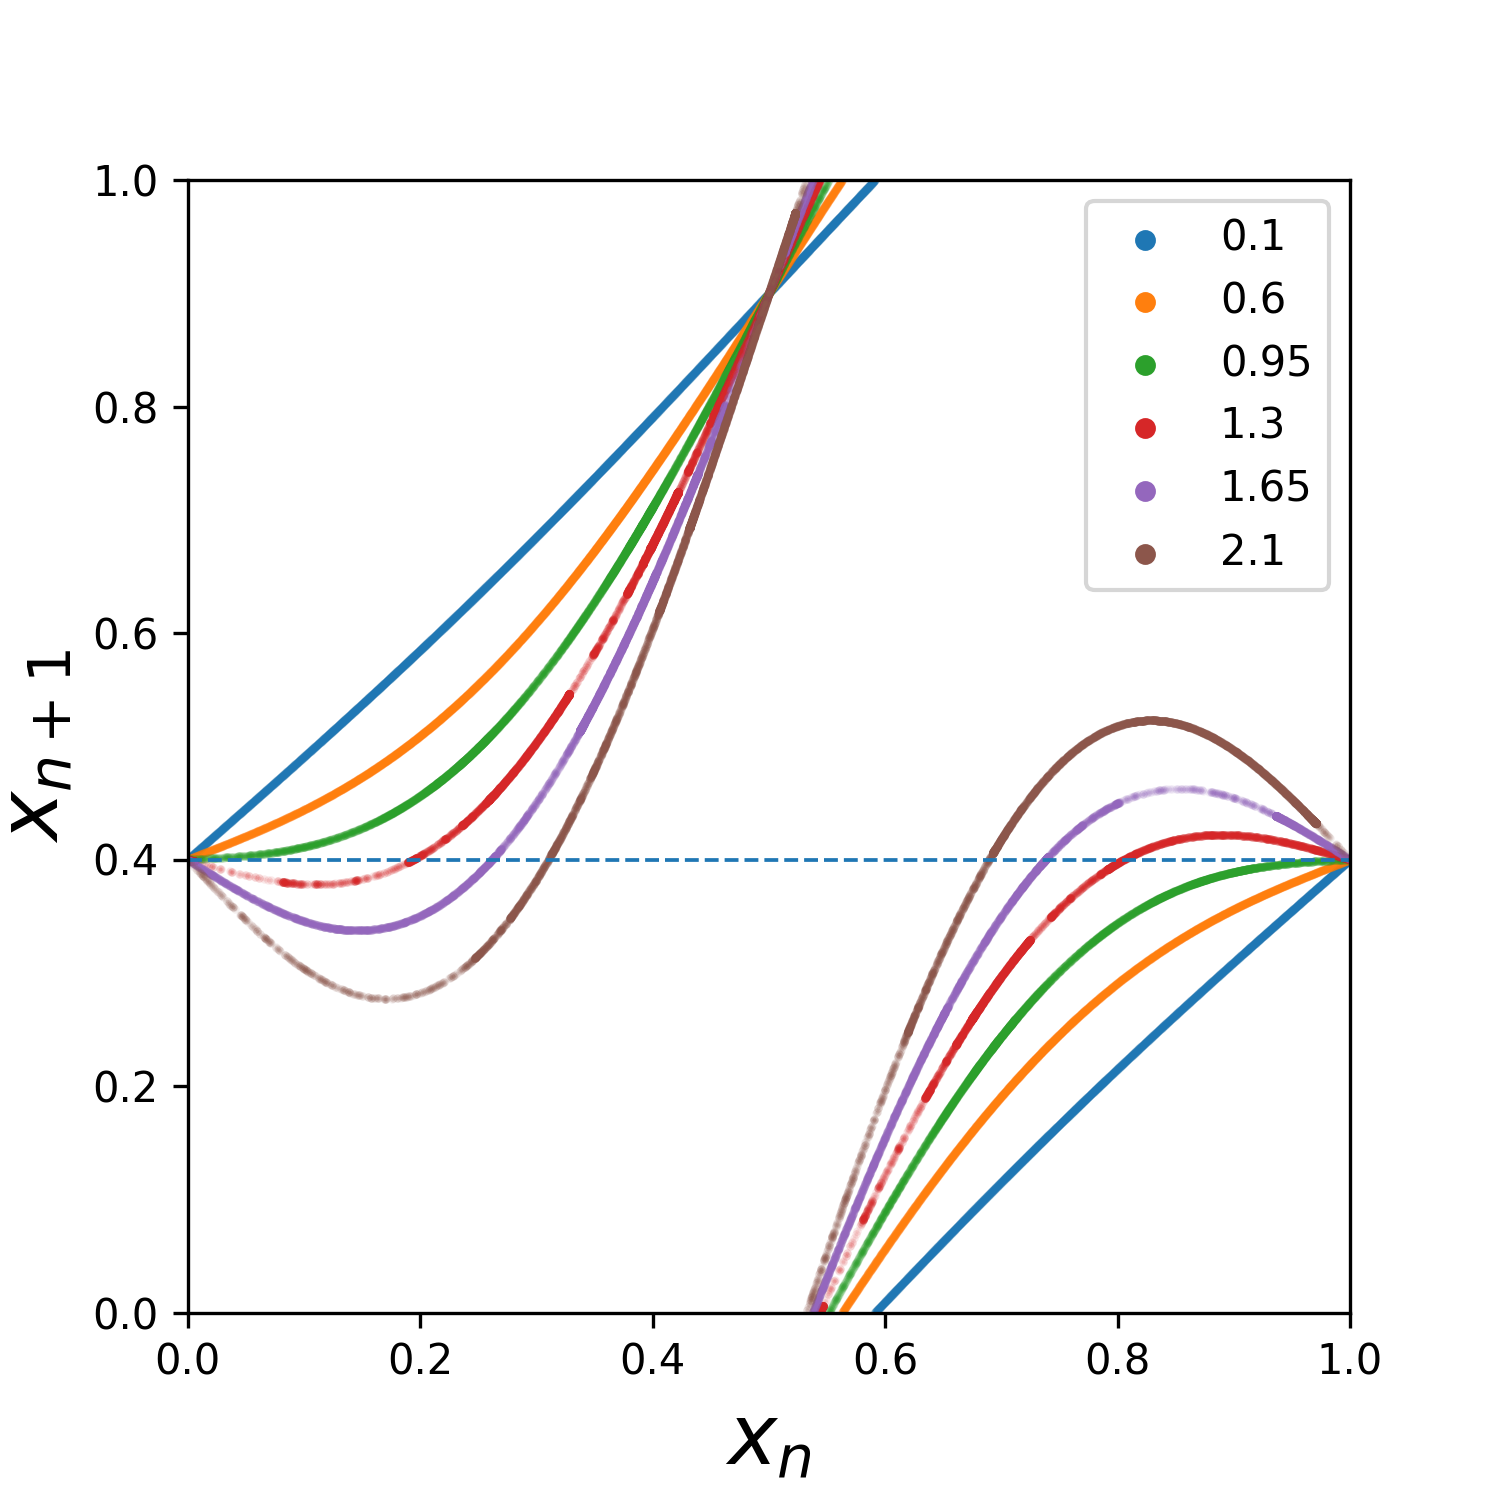
\includegraphics[width=0.3\textwidth]{../figures/chap1/4_3_py.png}
	   \caption{\scriptsize Mappa di Arnold al variare di $k$ con $\omega  = 0.4$ fissato.}
           \label{fig:4_3_py-png}
       \end{figure}
       \noindent
       Come possiamo vedere in figura \ref{fig:4_3_py-png} la mappa non è invertibile per tutti i valori di $k$. \\
       Prendiamo ad esempio la mappa con $k=0.1$ e valutiamo\
       \footnote{Questa corrisponde (circa) alla circle rotation map} il punto $x_n=0$: la linea blu in figura \ref{fig:4_3_py-png}, che rappresenta la mappa, a destra di questo punto vale $\omega+\epsilon$, a sinistra di questo punto vale $\omega-\epsilon$. La pendenza della curva in questo punto è quindi positiva.\\
       La presenza della perturbazione oscillante fa si che i due "rami" della mappa si avvicinino l'un l'altro "distorcendosi", di conseguenza se la perturbazione è abbastanza forte è possibile che in un punto tra $0$ e $1$ il ramo in alto e quello in basso abbiano la stessa $x_{n+1}$: si perde l'iniettività e quindi l'invertibilità.\\
       Nel grafico la perdita di iniettività si ha quando la mappa oltrepassa la linea tratteggiata (che rappresenta la separatrice tra i rami).\\
       Per capire quando questo succede possiamo studiare la pendenza della mappa nei pressi di $x_n = 0$ (considerandola di fatto come una funzione continua).
       \[
	   x_{n+1} = x_n + \omega + k x_n = (1-k) x_n + \omega
       .\] 
       Se in un intorno (destro) di questo punto la pendenza della curva è negativa allora significa che la mappa è scesa sotto $\omega$ e quindi ha perso l'iniettività: deve essere $k\le 1$ per avere pendenza positiva.



\begin{ex}[Applicazione delle forme di Jordan]
    Dato il sistema dinamico 
    \[
	\frac{\text{d} \vect{x}}{\text{d} t} = A\vect{x}  \quad \vect{x}\in \mathbb{R}^2, A = \begin{pmatrix} -1 & -1 \\ 1 & - 1 \end{pmatrix} 
    \] 
    \begin{itemize}
        \item Trovare la soluzione.
	\item Disegnare il Phase Portrait.
    \end{itemize}
\end{ex}
\noindent
\begin{ex}[]
    Sia $A$ una matrice $2\times 2$ reale. Supponiamo che $A$ abbia $2$ autovalori complessi coniugati: 
    \[
        \Lambda_1, \Lambda_2 = a \pm ib \quad b\neq 0
    \] 
    Dimostrare che esiste una matrice invertibile $P$ tale che:
    \[
	P^{-1}AP = \begin{pmatrix} a & b \\ -b & a \end{pmatrix} 
    \] 
\end{ex}
\noindent

\setcounter{section}{6}
\section{Sistemi lineari in dimensione $n$}%
\begin{ex}[Base di autovettori generalizzati]
Sia data 
\[
    A = 
    \begin{pmatrix} 
	6 & 2 & 1 \\
	- 7 & -3 & -1 \\
	-11 & -7 & 0 
    \end{pmatrix} 
.\] 	
Determinare una base di autovettori generalizzati di $A$.
\end{ex}
\noindent
\begin{ex}[Soluzione sistema in $\mathbb{R}^4$ (1)]
\[
    \frac{\text{d} \v{x}}{\text{d} t} = A \v{x}, \qquad \v{x}(0) = \v{x}_0 \in R^4, \quad A = 
    \begin{pmatrix} 
	0 & -2 & -1 & -1 \\
	1 & 2 & 1 & 1 \\
	0 & 1 & 1 & 0 \\
	0 & 0 & 0 & 1
    \end{pmatrix} 
.\] 	
\end{ex}
\noindent
 
\begin{ex}[Soluzione di sistema in $\mathbb{R}^4$ (2)]
Risolvere il seguente IVP:
\[
    \frac{\text{d} \v{x}}{\text{d} t} = A \v{x} \qquad A = 
    \begin{pmatrix}   
	0 & -1 & 0 & 0 \\
	1 & 0 & 0 & 0 \\
	0 & 0 & 0 & -1 	\\
	2 & 0 & 1 & 0 
    \end{pmatrix} 
.\] 
\end{ex}
\noindent

\begin{ex}[Autovettori generalizzati ed autovalori]
Dato l'IVP in $R^4$:
\[
    \frac{\text{d} \v{x}}{\text{d} t} = A \v{x}
.\] 
con 
\[
    A = 
    \begin{pmatrix}
	0 & -1 & 0 & 0\\
	1 & 0 & 0 & 0 \\
	0 & 0 & 0 & -1\\
	2 & 0 & 1 & 0
    \end{pmatrix} 
.\] 
Trovare gli autovettori generalizzati e gli autovalori.
\end{ex}
\noindent

\section{Manifold lineari, stabile, instabile e centro}%
\begin{ex}[]
    Dimostrare che ogni stato stazionario dell'esercizio
    \[
        \frac{\text{d} \v{x}}{\text{d} t} = A \v{x} \quad  \v{x}\in \mathbb{R}^2 \quad
	A = 
    \begin{pmatrix}
	0  & 1 \\
	0 & -4 \\
    \end{pmatrix}
    .\] 
    Che abbiamo dimostrato essere della forma: $\begin{pmatrix} x_s \\ 0 \end{pmatrix} $ è stabile secondo Lyapunov (non bisogna usare gli autovalori, utilizzare la tecnologia della definizione di Lyapunov).
\end{ex}
\noindent
\begin{ex}[]
    Dato il sistema dinamico con matrice $A$:
    \[
        A = 
    \begin{pmatrix}
	-2 & -1 & 0 \\
	1 & -2 & 0 \\
	0 & 0 & 3 \\
    \end{pmatrix}
    .\] 
    Oppure 
    \[
        A = 
    \begin{pmatrix}
	0 & -1 & 0 \\
	1 & 0 & 0 \\
	0 & 0 & 2 \\
    \end{pmatrix}
    .\] 
    Determinare $E^s, E^u, E^c$.
\end{ex}
\noindent
\begin{ex}[]
    Dato il sistema dinamico 
     \[
        \frac{\text{d} \v{x}}{\text{d} t} = A \v{x} \quad  \v{x}\in \mathbb{R}^2 \quad  A = 
    \begin{pmatrix}
	-1 & -3 \\
	-3 & -1 \\
    \end{pmatrix}
    .\] 
    Sia $H:\mathbb{R}^2\to \mathbb{R}^2 $  tale che:
    \[
        \forall \v{v} = \begin{pmatrix} x \\ y \end{pmatrix} \in \mathbb{R}^2: \ \v{v}\to H\v{v}
    .\] 
    Con:
    \[
        H = \frac{1}{\sqrt{2} } 
    \begin{pmatrix}
	1 & -1 \\
	1 & 1 \\
    \end{pmatrix}
    .\]  
    Determinare come viene trasformato il SD attraverso $H$.
\end{ex}
\noindent


\end{document}
